\documentclass[12pt,a4paper]{amsart}

\usepackage[slovene]{babel}
\usepackage[utf8]{inputenc}
\usepackage{amsmath,amssymb,amsfonts,bm}
\usepackage{url}
\usepackage{graphicx,subfig}




\textwidth 15cm
\textheight 24cm
\oddsidemargin.5cm
\evensidemargin.5cm
\topmargin-5mm
\addtolength{\footskip}{10pt}
\pagestyle{plain}
\overfullrule=15pt

\theoremstyle{definition}
\newtheorem{definicija}{Definicija}[section]
\newtheorem{primer}[definicija]{Primer}
\newtheorem{opomba}[definicija]{Opomba}

\theoremstyle{plain}
\newtheorem{lema}[definicija]{Lema}
\newtheorem{izrek}[definicija]{Izrek}
\newtheorem{trditev}[definicija]{Trditev}
\newtheorem{posledica}[definicija]{Posledica}

\newcommand{\N}{\mathbb N}
\newcommand{\R}{\mathbb R}

\begin{document}

% Naslovnica
%----------------------------------------------------------------------------------------------------
\thispagestyle{empty}
\noindent{\large
Univerza v Ljubljani\\[1mm]
Fakulteta za matematiko in fiziko\\[3mm]
Finančna matematika -- 1.~stopnja}
\vfill

\begin{center}{\large
Tilen Humar, Urban Rupnik\\[2mm]
{\Huge \bf Iskanje bitonične rešitve problema potujočega trgovca}\\[5mm]
Projekt OR pri predmetu Finančni praktikum\\[1cm]}
\end{center}
\vfill

\noindent{\large
Ljubljana, 2022}
\pagebreak

%----------------------------------------------------------------------------------------------------
\section{Predstavitev problema}

\noindent
{\bf Problem potujočega trgovca} oziroma {\bf problem trgovskega potnika} je ponavadi zastavljen v 
naslednji obliki.
\newline

\noindent
Obstaja $n$ mest, za katera poznamo razdalje med poljubnim parom mest. Trgovec želi obiskati vsa mesta, 
pri čemer pot začne in konča v istem mestu in vsak kraj obišče natanko enkrat. Katera je najkrajša 
oziroma najcenejša pot, ki jo lahko izbere trgovec?
\newline

\noindent
V matematičnem jeziku se problem torej prevede na iskanje najcenejšega Hamiltonovega cikla v polnem 
grafu $K_n$, kjer ima vsaka povezava $e$ znano utež (ceno) $c_e$. Ker pa je v osnovi dotični problem
``NP-težek'', to je, da bi za iskanje njegove rešitve potrebovali več kot polinomski čas, se omejimo na
lažjo nalogo iskanja njegove najkrajše bitonične rešitve.
\newline

\section{Bitonična pot}

\begin{definicija}
    Zaporedje $(x_n)_{n \in \N}$ je bitonično, ko obstaja tak $k, 1 \leq k < n$, da velja
    $$x_1 \leq x_2 \leq \cdots \leq x_k \geq \cdots \geq x_n.$$
\end{definicija}

\noindent
Bitonična rešitev problema, bo torej pot, kjer bomo začeli v skrajno levo ležečem vozlišču, nadaljevali strogo
desno do najbolj desnega vozlišča in še strogo levo nazaj do izhodišča. Bitoničnost poti lahko na grafu 
preverimo z navpičnicami. Vsaka navpična črta seka pot največ dvakrat.


\begin{figure}[!htb]%
    \centering
    \subfloat[\centering Bitonična pot]{{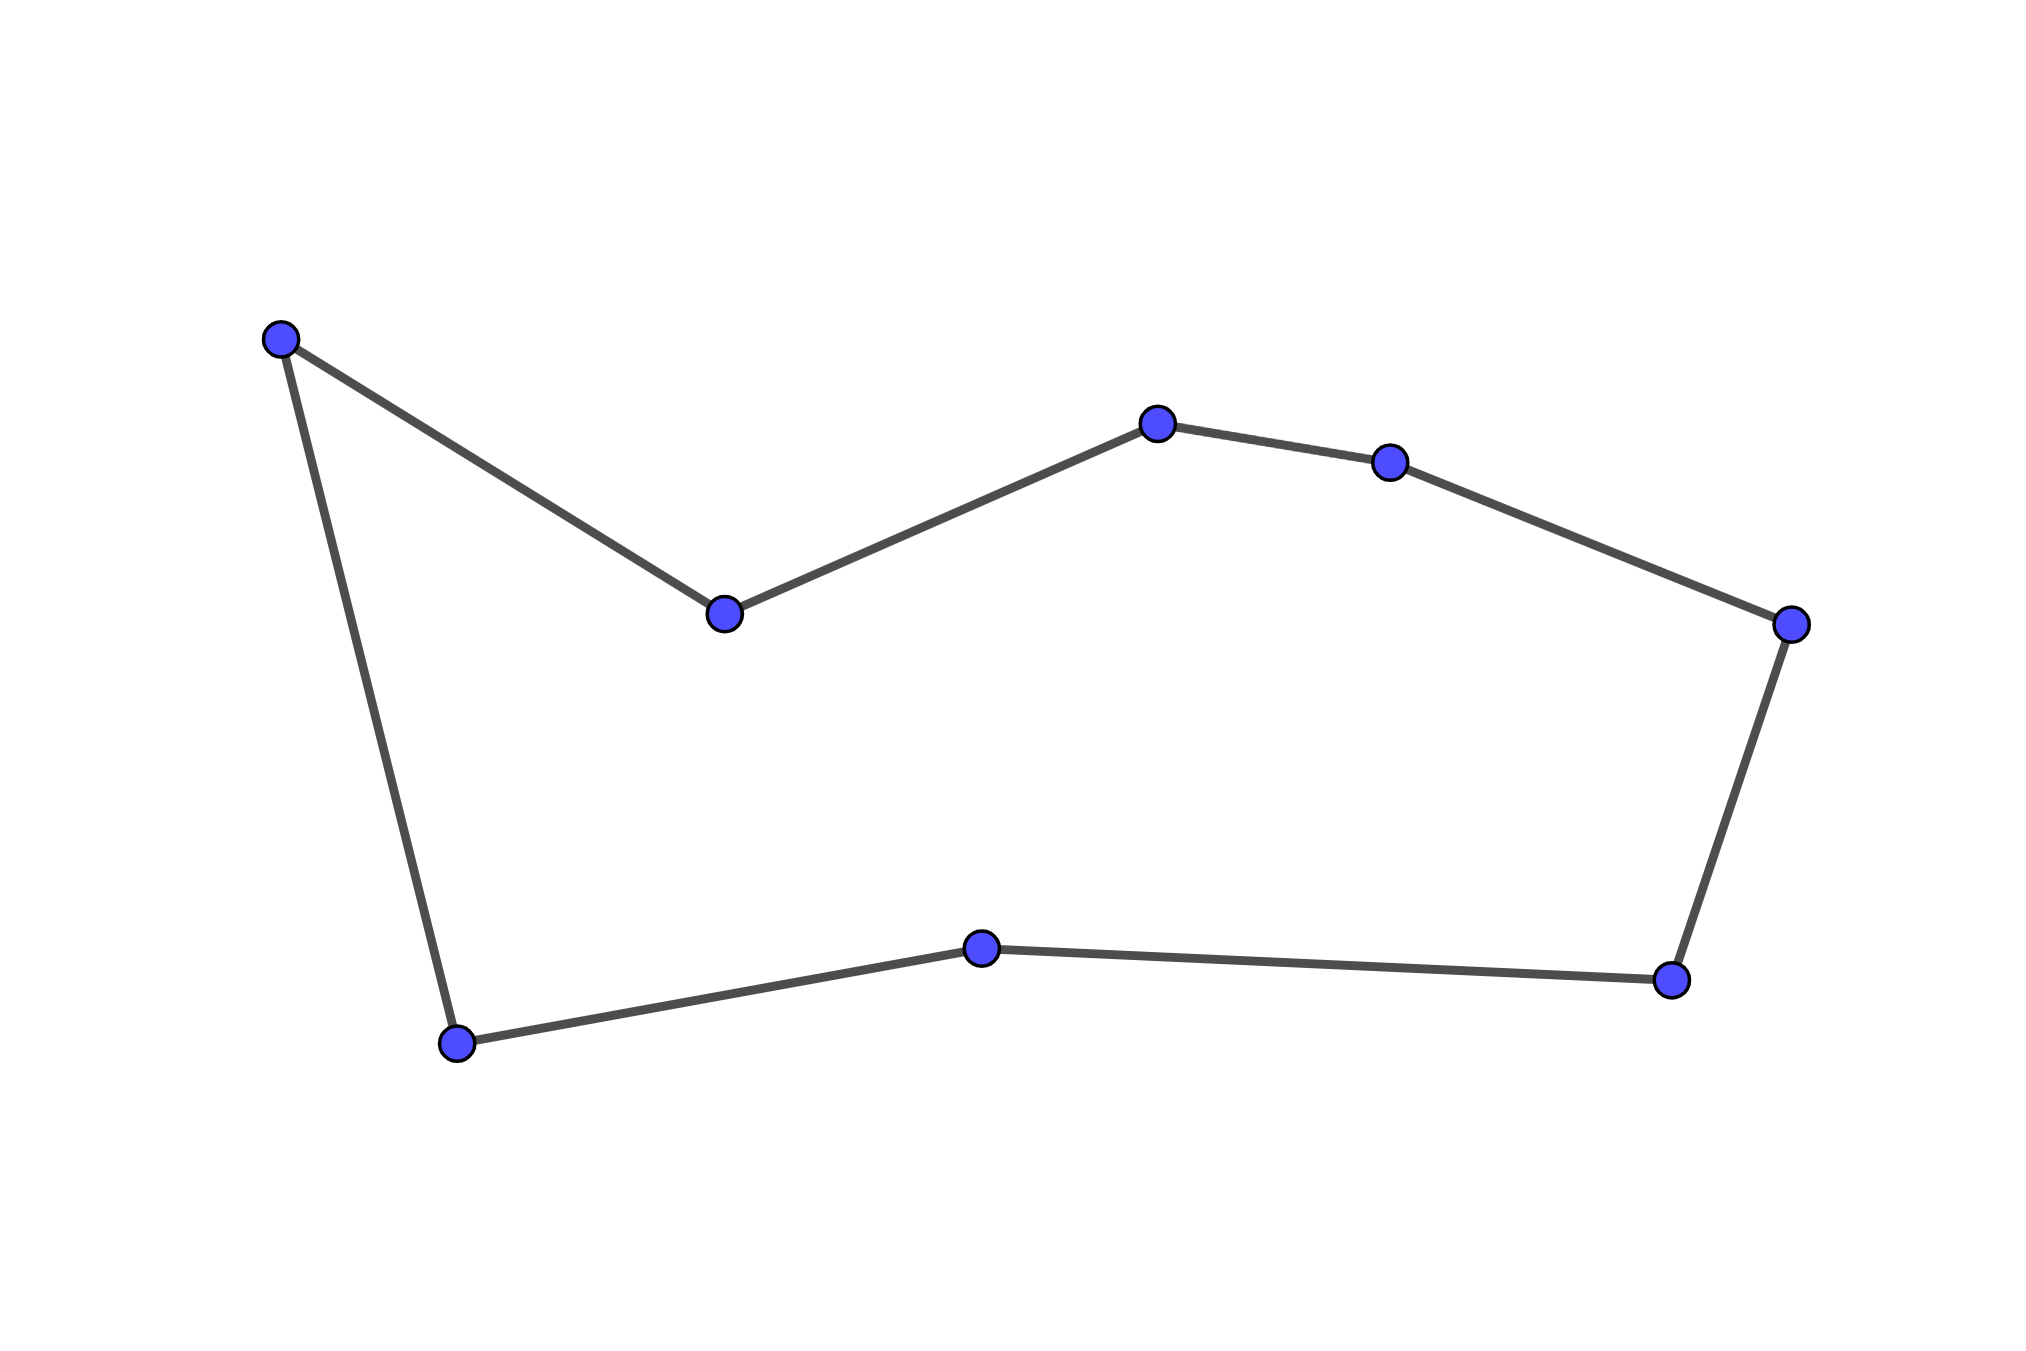
\includegraphics[width=6.9cm]{Slike grafov/graf1.png} }}%
    \qquad
    \subfloat[\centering Nebitonična pot]{{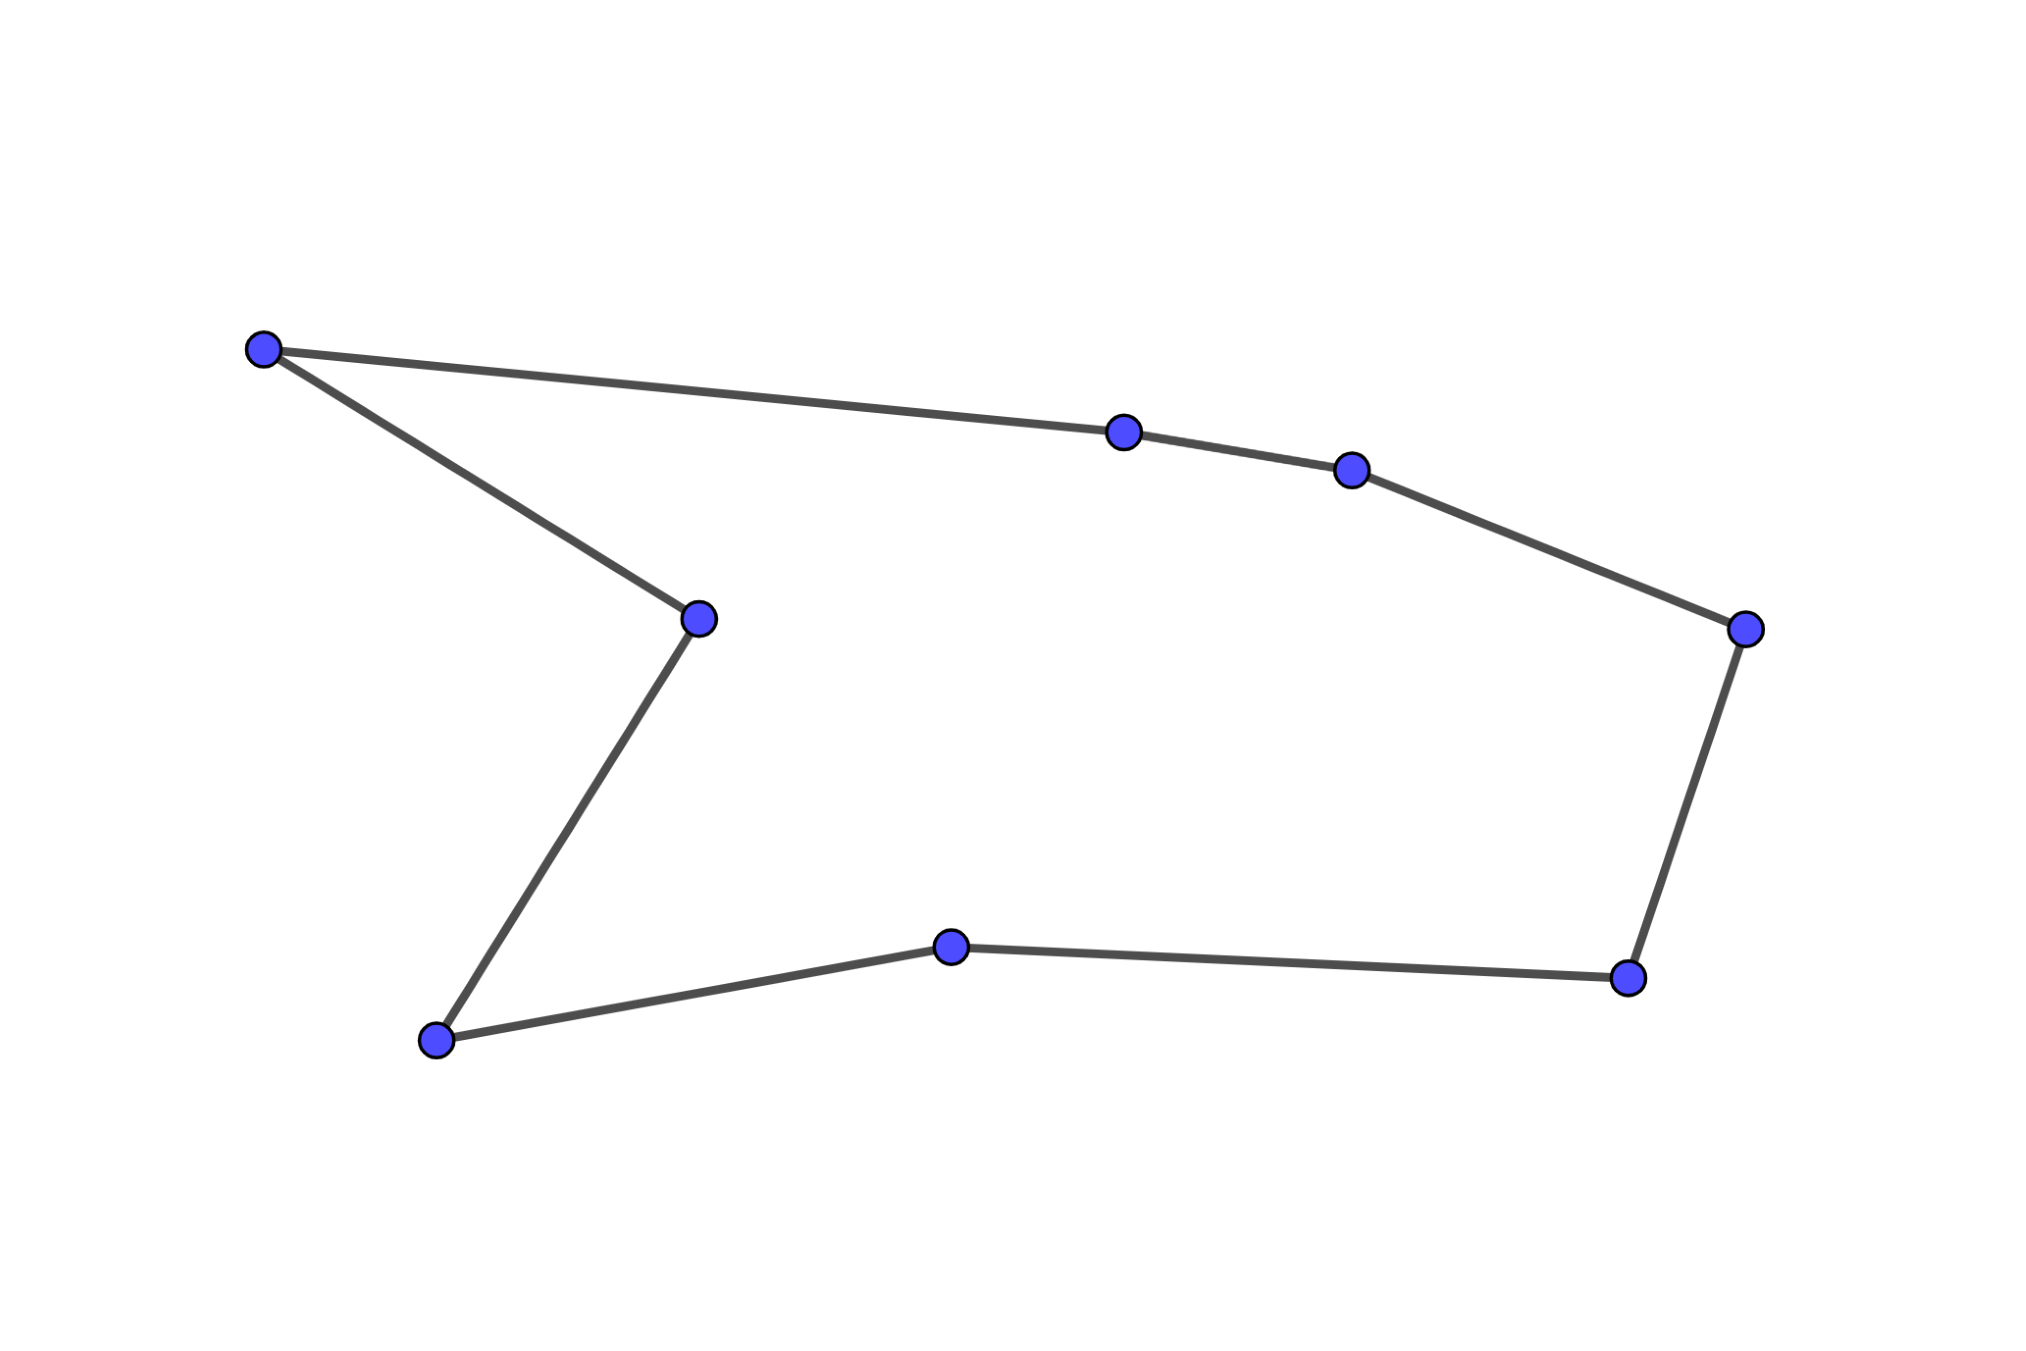
\includegraphics[width=6.9cm]{Slike grafov/graf2.png} }}%
    \caption{Primer bitonične in nebitonične poti na grafu}%
    \label{fig:example}%
\end{figure}


\noindent
Iskanje najkrajše bitonične poti je standardna naloga v dinamičnem programiranju, rešljiva v polinomskem
času $O(n^2),$ poznamo pa tudi hitrejši algoritem s časovno zahtevnostjo $O(n \log^2 n).$
\newline

\newpage
\section{Načrt dela}

\noindent
Za iskanje rešitev problema bova pripravila program v programskem jeziku R. 
Ta bo okvirno vseboval:

\begin{itemize}
    \item funkcijo za generiranje točk v $\R^2$ (predpostavka: $x$ koordinate so različna
    naravna števila, $y$ pa poljubna realna)
    \item funkcijo za risanje točk
    \item funkcijo za izračun evklidske razdalje med točkama
    \item program za iskanje najkrajše bitonične poti
    \item funkcijo za izpis poti
\end{itemize}

\noindent
Nato sledi še eksperimentiranje z napisanim programom.

\end{document}